\chapter{Implementation}\label{chap:implementation}
\begin{spacing}{1.2}
\minitoc
\thispagestyle{MyStyle}
\end{spacing}
\newpage

\section*{INTRODUCTION}
\addcontentsline{toc}{section}{INTRODUCTION}
This chapter details the programmatic implementation of the architecture formulated in Chapter~\ref{chap:architecture}. It examines the concrete realization of the BACAB layered pattern across the backend microservices, the deterministic lifecycle mechanics of the manager service, the per-turn pipeline orchestration of the copilot service, the parsing logic of the intelligence service, and the integration via the user interface. Implementation status is rigorously classified: operational and tested capabilities are documented as such, architecturally specified but unconnected interfaces are explicitly identified, and features relegated to future scope are strictly excluded from current achievements.

\section{Development Environment and Toolchain}\label{sec:impl_env}
The three backend microservices are developed using Python~3.11 and the FastAPI~0.115 framework. SQLAlchemy~2 provides the Object-Relational Mapping (ORM) layer, while Pydantic~2 enforces strict boundary validation, with the translator layer mediating data transfer objects between them. The user interface is built as a single-page application utilizing TypeScript, Next.js~15, and React~18, styled via Tailwind CSS and the shadcn/ui component library.

The manager and intelligence services utilize PostgreSQL for relational persistence; the copilot employs SQLite for development-mode persistence of conversational threads, turn metadata, and execution records. The copilot's probabilistic language-model invocations interface with Azure OpenAI, with dynamic model selection governed by environment variables. Source code is versioned using Git within a polyrepo-in-monorepo structure. Containerization and Continuous Integration (CI) maturity vary across the platform, as codified in Table~\ref{tab:toolchain}.

\begin{table}[H]
\centering
\scriptsize
\renewcommand{\arraystretch}{1.3}
\begin{tabular}{|p{3.4cm}|p{4.6cm}|p{6cm}|}
\hline
\rowcolor{lightgray}
\textbf{Architectural Layer} & \textbf{Technology Stack} & \textbf{Operational Role} \\ \hline
Backend Services & Python 3.11 / FastAPI 0.115 / SQLAlchemy 2 / Pydantic 2 & Core programming language, high-performance web framework, ORM engine, and boundary schema validation. \\ \hline
Frontend & Next.js 15 / React 18 / TypeScript / Tailwind CSS / shadcn/ui & Client-side application framework, strong typing, declarative styling, and component library. \\ \hline
Data Stores & PostgreSQL + SQLite & PostgreSQL for deterministic state persistence (manager, intelligence); SQLite for localized copilot session memory. \\ \hline
External Integrations & Azure OpenAI API & Probabilistic generative backend for the copilot, securely invoked via injected deployment variables. \\ \hline
Containerization & Docker (Backend focus) & Isolated container images for backend APIs; UI service and unified root composition remain in development. \\ \hline
Development Tooling & Git (Polyrepo-in-monorepo) & Distributed source control and repository orchestration. \\ \hline
Continuous Integration & Manager service exclusively & Automated CI workflow deployed for the manager; extension to copilot, intelligence, and UI is a prioritized hardening objective. \\ \hline
\end{tabular}
\caption{Principal technological stack utilized for the implementation of the Itqan platform}
\label{tab:toolchain}
\end{table}

Table~\ref{tab:impl_evidence} synthesizes the implementation evidence substantiating the delivery of the four primary platform components.

\begin{table}[H]
\centering
\scriptsize
\renewcommand{\arraystretch}{1.3}
\begin{tabularx}{\linewidth}{|p{3cm}|>{\RaggedRight\arraybackslash}X|p{4cm}|}
\hline
\rowcolor{lightgray}
\textbf{Component} & \textbf{Implemented Scope} & \textbf{Validation Evidence} \\ \hline
\texttt{rfq\_manager\_ms} & RFQ lifecycle orchestration, workflow-derived pre-created staging, three-gate transactional advancement, granular subtasks, structured notes, file references, reminders, and analytical data endpoints. & 259 executed tests (100\% passing rate); validated OpenAPI contract; manual Postman integration checks. \\ \hline
\texttt{rfq\_copilot\_ms} & Trust-boundary pipeline architecture; operational Paths 1, 4, and the robust Path 8 safety fallback family; bounded working-memory capture; execution of guardrails and LLM Judge. & 636 executed tests (100\% passing rate); static anti-drift tests; formalized architecture specification. \\ \hline
\texttt{rfq\_intelligence\_ms} & Deterministic parsing foundation for Material Requisition (MR) packages and complex workbooks; heuristic anomaly detection; briefing artifact foundation and briefing assembly in progress. & 118 collected tests; 64 passing, 48 fixture-dependent (golden artifacts excluded from Git), 6 skipped. \\ \hline
\texttt{rfq\_ui\_ms} & Portfolio visualization, RFQ detail interface, copilot conversational drawer, dashboard analytics, and intelligence artifact panels. & 12 source-contract validation scripts (11 passing); UI demonstrability within the current prototype scope. \\ \hline
\end{tabularx}
\caption{Implementation evidence synthesis across delivered platform components (test counts derived from the project snapshot detailed in Appendix~\ref{app:test-evidence})}
\label{tab:impl_evidence}
\end{table}

\subsection{BACAB Discipline Across the Backend Services}
All three backend microservices rigorously implement the BACAB layered pattern (Chapter~\ref{chap:architecture}, Section~\ref{sec:bacab_pattern}) as their foundational software architecture. The manager service is detailed subsequently as the most mature instantiation; the intelligence service strictly mirrors this topology; and the copilot service inherits the BACAB skeleton while injecting a dedicated \texttt{pipeline} module to orchestrate the per-turn stages defined in Chapter~\ref{chap:architecture}.

\section{Manager Service Implementation}\label{sec:manager_impl}
The manager service functions as the operational hub of the platform. Its implementation encompasses RFQ registration, workflow-driven lifecycle staging, transactional stage progression, hierarchical subtasks, immutable notes, file telemetry, reminder execution, audit-history scaffolding, and analytical aggregation.

\subsection{BACAB Topology within the Manager Service}\label{sec:manager_bacab}
The manager service operationalizes the BACAB pattern via a strict directory taxonomy that reflects the active-and-support layer dichotomy. A specific programmatic deviation consolidates Pydantic request/response schemas alongside translator mapping functions within the \texttt{translators} layer, rather than isolating them. Each Python module maps exactly to a designated architectural layer. The three invariant discipline rules (Chapter~\ref{chap:architecture}, Section~\ref{sec:bacab_pattern}) are absolute, enforced structurally by linting constraints and CI workflow policies. Listing~\ref{lst:manager_tree} illustrates this topological layout.

\begin{lstlisting}[basicstyle=\ttfamily\footnotesize, frame=single, captionpos=b, label={lst:manager_tree}, caption={Topological BACAB layout of \texttt{rfq\_manager\_ms} (depth 2)}]
rfq_manager_ms/
+-- src/
|   +-- controllers/   # Domain orchestration logic (6 modules)
|   +-- routes/        # HTTP ingress and validation (6 modules)
|   +-- datasources/   # ORM abstraction and queries (6 modules)
|   +-- models/        # SQLAlchemy relational entities (12 tables)
|   +-- translators/   # DTO schemas and mapping logic
|   +-- connectors/    # External system integration (event_bus, IAM)
|   +-- services/      # Cross-cutting operational logic
|   +-- config/, utils/
+-- migrations/        # Alembic schema versioning
+-- tests/             # Pytest automated suite (259 passing tests)
\end{lstlisting}

\subsection{Relational Schema and Stage Progression}\label{sec:db_schema}
The persistence layer comprises twelve relational tables hosted in PostgreSQL. The seven primary entities of the domain model (RFQ, Workflow, RFQ\_Stage, Subtask, Note, File, Reminder) translate symmetrically (1:1) into SQLAlchemy ORM models. Five auxiliary tables support complex state management: \texttt{stage\_template}, \texttt{rfq\_stage\_field\_value}, \texttt{reminder\_rule}, \texttt{rfq\_code\_counter}, and the reserved \texttt{rfq\_history} audit table.

Lifecycle progression synthesizes the three theoretical gates (mandatory-field, blocker, transition-validity) into a singular, ACID-compliant database transaction. Each gate evaluates distinct criteria; failure at any gate halts the process, yielding a structured exception detailing the exact constraint violation. Upon unanimous validation, the transaction commits atomically: the current stage is marked as completed with an actual end timestamp, the next pre-created stage in the workflow sequence is activated, and completion metrics are recalculated. This guarantees that the RFQ lifecycle never enters an inconsistent or partial state. Lifecycle traceability relies inherently on chronological timestamps, persisted stage states, append-only constraints on notes, and non-destructive entity updates. Listing~\ref{lst:advance_stage} demonstrates the HTTP route interface executing this transactional progression.

\begin{lstlisting}[language=Python, basicstyle=\ttfamily\footnotesize, frame=single, breaklines=true, captionpos=b, label={lst:advance_stage}, caption={Representative HTTP endpoint executing the three-gate stage advancement transaction. (Note: Dependency injection and error handling obfuscated for brevity).}]
# routes/rfq_stage_route.py  (representative excerpt)
@router.post("/rfqs/{rfq_id}/stages/{stage_id}/advance")
def advance_stage(rfq_id: UUID, stage_id: UUID, ...):
    # Controller orchestrates a singular ACID transaction:
    #   1. Mandatory-field gate: Validates completeness 
    #      of required inputs.
    #   2. Blocker gate: Confirms resolution of all 
    #      blocking constraints.
    #   3. Transition-validity gate: Verifies target 
    #      against canonical workflow.
    # Upon unanimous success: completes current stage,
    # activates the next pre-created stage, updates metrics.
    # Upon failure: rolls back transaction, 
    # returns structured constraint exception.
    return controller.advance(rfq_id, stage_id, ...)
\end{lstlisting}

\subsection{Subtasks, Notes, Files, and Reminders}\label{sec:manager_resources}
Four subsidiary resource models complement the core lifecycle architecture. \textbf{Subtasks} function as granular execution increments attached to specific stages, implementing soft-delete semantics: deprecated subtasks are timestamped and retained, while being excluded from recursive progress calculations. \textbf{Notes} enforce strict append-only constraints: the API exposes solely \texttt{POST} and \texttt{GET} methods, structurally prohibiting \texttt{PUT} and \texttt{DELETE} operations to preserve the integrity of the communication audit trail. \textbf{Files} represent binary object references, explicitly categorized by MIME type; this includes a designated estimation workbook type primed for deterministic parsing by the intelligence service (autonomous event-driven consumption is architecturally prepared but currently inactive). \textbf{Reminders} constitute temporal execution triggers, supporting both manual instantiation and rule-based generation.

\subsection{Analytics and Telemetry Endpoints}\label{sec:manager_analytics}
The manager service provides a robust analytical interface, aggregating operational RFQ data via two primary REST endpoints: \texttt{/rfqs/stats} computes high-level portfolio KPIs (aggregate volume, active queue size, critical path flags, and mean cycle time), while \texttt{/rfqs/analytics} delivers multi-dimensional win-rate breakdowns (terminal status categorization aggregated by client or workflow template). Advanced financial analytics (margin analysis and estimation accuracy) require longitudinal outcome data currently outside the system's capture parameters, and are consequently deferred to future development phases.

\subsection{Observability and Audit-History Implementation}\label{sec:manager_observability}
The manager service is packaged via a Dockerfile and orchestrated through a scenario-specific docker-compose configuration. The service emits structured telemetry, injecting correlation identifiers into request headers to facilitate distributed tracing across routes, controllers, and datasources. Enhancing cross-service identifier propagation remains a critical observability objective. System health is monitored via standard \texttt{/health} liveness probes and a \texttt{/metrics} endpoint instrumented via the official Prometheus client.

Crucially, the database schema implements an \texttt{rfq\_history} table designed to capture generic, immutable audit logs across all lifecycle entities. However, no active write paths currently populate this table (a deliberate architectural constraint formalized in Architectural Decision Record H5). Lifecycle traceability currently relies on implicit temporal state variables; the activation of explicit audit logging is flagged as a high-priority hardening requirement.

\section{Copilot Service Implementation}\label{sec:copilot_impl}
The copilot codebase is engineered across two parallel release lanes: a \textbf{v1 lane} that established the foundational conversational interfaces, and a \textbf{v2 lane} that rigorously implements the deterministic trust-boundary architecture (Chapter~\ref{chap:architecture}). The most recent operational slice finalized v2 thread management and bounded working-memory capture. Consequently, the v2 trust-boundary pipeline is the execution path for every conversational turn, while the v1 thread-management routes remain mounted and are still consumed by the frontend (the thread-lifecycle cutover remains a pending alignment task).

Structurally, v2 leverages the BACAB paradigm, isolating a distinct \texttt{pipeline} layer between the controllers and data access objects. This layer encapsulates every discrete execution stage (Intake, Planner, Validator, Factory, Resolver, Access, Tool Executor, Evidence Check, Context Builder, Compose, Guardrails, Judge, Escalation Gate, Finalizer, and Persist) as independent Python modules, orchestrating them sequentially via the primary turn controller.

\subsection{Turn Processing Pipeline and Vertical Slicing}
A user query initiates a strictly linear sequence of execution stages. Each stage is responsible for a singular decision matrix: \textbf{FastIntake $\rightarrow$ LLM Planner $\rightarrow$ PlannerValidator $\rightarrow$ ExecutionPlanFactory $\rightarrow$ Resolver $\rightarrow$ Access (manager-mediated authorization) $\rightarrow$ Tool Executor $\rightarrow$ Evidence Check $\rightarrow$ Context Builder $\rightarrow$ Compose $\rightarrow$ Guardrails $\rightarrow$ Judge $\rightarrow$ Finalizer $\rightarrow$ Persist}. Working memory is loaded into the execution state by the turn controller after plan construction, explicitly preserving the ExecutionPlanFactory's isolation; in the current slice it is not injected into the Planner, Compose, or Judge prompts. This sequence corresponds to the canonical pipeline conceptualized in Chapter~\ref{chap:architecture} (Figure~\ref{fig:canonical_pipeline}), which distinguishes deterministic programmatic execution from probabilistic LLM invocations.

The initial vertical slice validates three critical execution paths end-to-end: \textbf{Path~1} (Deterministic intake routing for trivial conversational inputs), \textbf{Path~4} (The core operational capability executing evidence-grounded RFQ queries via authorized manager connectors), and the robust \textbf{Path~8} safety matrix handling five distinct failure modes. Capabilities designated as Paths 2, 3, 5, 6, and 7 are architecturally defined but systematically routed to Path 8.1 (Unsupported Operation) via the Escalation Gate pending their respective implementations.

\subsection{Path Registry and Single-Construction Invariance}
The \textbf{Path Registry} functions as the declarative policy matrix, parsed at runtime exclusively by the ExecutionPlanFactory and the Escalation Gate. The \textbf{Planner} leverages a structured Azure OpenAI invocation, constrained by JSON schema, to probabilistically classify intent. The \textbf{PlannerValidator} enforces structural and schema integrity on this output, operating strictly without referencing the policy registry.

The \textbf{ExecutionPlanFactory} serves as the absolute architectural chokepoint, uniquely authorized to instantiate a \texttt{TurnExecutionPlan}. Three fundamental architectural invariants are aggressively enforced via static syntax-tree (anti-drift) tests within the copilot's automated test suite: (1) \textit{Single-Construction Anomaly Detection}, ensuring no external code instantiates the execution plan; (2) \textit{Registry-Reader Whitelisting}, restricting Path Registry access exclusively to authorized components; (3) \textit{Deterministic Intake Enforcement}, demanding that FastIntake executes solely via anchored regex evaluations devoid of network or LLM latency. 

\subsection{Memory, Guardrails, and the Escalation Gate}
The working memory sub-system currently operates in a capture-only paradigm: contextual turn data is persisted but not recursively injected into the generative prompt (an isolation enforced by anti-drift testing). The \textbf{Guardrails} layer executes deterministic validation on the generated response (validating evidence grounding and schema conformity). The \textbf{Judge} component initiates a secondary, constrained LLM invocation to classify the generated text against severe anomalies (fabrication, unauthorized inference).

The \textbf{Escalation Gate} acts as the universal deterministic intercept mechanism for pipeline failures. It algorithmically maps any exception (e.g., target obfuscation, evidence sparsity, guardrail failure) to a corresponding Path 8 protocol, dynamically re-routing execution back through the factory to synthesize a safe, structured degradation response rather than throwing a raw system exception. Crucially, the Gate never constructs a plan itself: it raises a structured \texttt{EscalationRequest} and re-enters \texttt{ExecutionPlanFactory.build\_from\_escalation()}, preserving the single-construction invariant even on the failure path. The trigger determines the target sub-case among the five members of the Path 8 family (8.1 unsupported/invalid, 8.2 out-of-scope, 8.3 clarification, 8.4 inaccessible, 8.5 no-evidence/service-unavailable), while the \texttt{reason\_code} selects the specific safe-response template rendered by the Finalizer (Figure~\ref{fig:escalation_gate}).

\begin{figure}[H]
    \centering
    \setlength{\fboxsep}{5pt}
    \setlength{\fboxrule}{0.5pt}
    \fbox{
        \IfFileExists{images/fig_5_1_escalation_gate.png}{%
            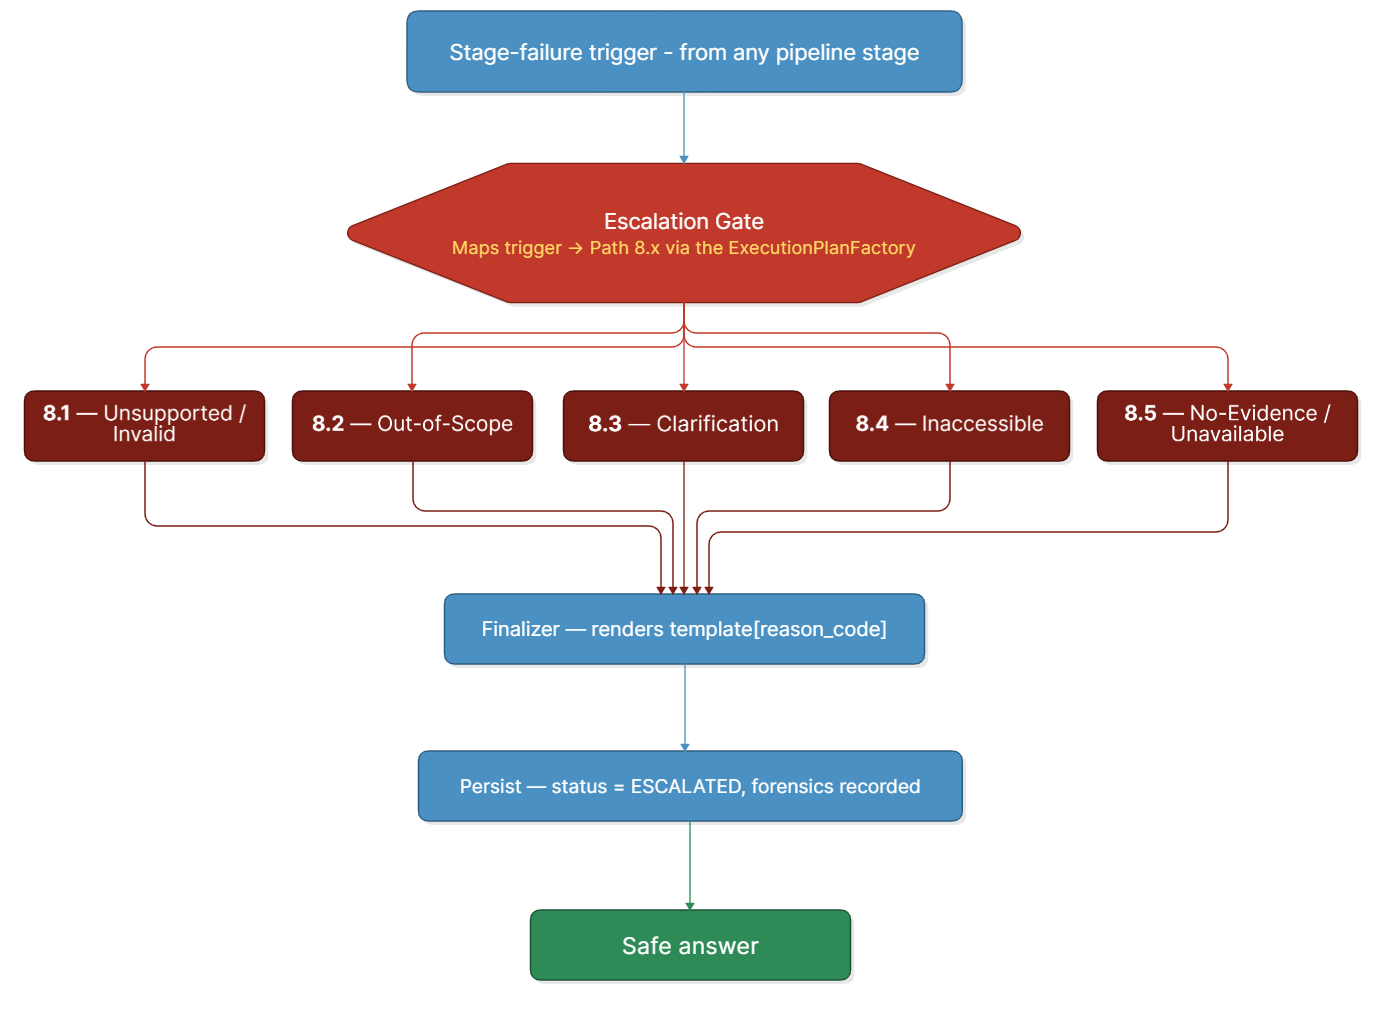
\includegraphics[width=\linewidth]{images/fig_5_1_escalation_gate.png}%
        }{%
            \begin{minipage}[c][8cm][c]{14cm}
                \centering
                \textit{[Figure 5.1 placeholder: the Escalation Gate and the Path 8 safety family. A failure trigger raised by any pipeline stage is intercepted by the deterministic Escalation Gate, which re-enters the ExecutionPlanFactory to construct a Path 8.x plan; the trigger selects the sub-case (8.1 unsupported, 8.2 out-of-scope, 8.3 clarification, 8.4 inaccessible, 8.5 no-evidence/unavailable) and the reason code selects the Finalizer template, yielding a safe answer with forensics persisted.]}
            \end{minipage}%
        }
    }
    \caption{The Escalation Gate and the Path 8 safety family: any stage-failure trigger is deterministically mapped, via a single re-entry into the \texttt{ExecutionPlanFactory}, to one of five Path 8.x safe-degradation responses, with the reason code selecting the rendered template}
    \label{fig:escalation_gate}
\end{figure}

\section{Intelligence Service Implementation}\label{sec:impl_intelligence}
The intelligence service is implemented as a specialized FastAPI module adhering to the identical BACAB architecture, organizing extracted artifacts through a PostgreSQL-backed artifact model. The data model is structurally unified: a central \texttt{artifact} table stores polymorphic entities including MR package profiles, analytical workbook parameters, and automated briefings, indexed by RFQ identifier.

The \textbf{MR package parser} deterministically maps canonical document structures (e.g., benchmark SA-AYPP-6-MR-022) to extract material taxonomies, vendor constraints, and technical metadata. The \textbf{workbook parser} anchors extraction to a three-sheet signature set (\textit{General}, \textit{Bid~S}, \textit{Top Sheet}) within the 32-sheet GHI reference workbook (e.g., fixture IF-25144), extracting cost-related values and schedule-relevant parameters where supported by the workbook structure. Critically, anomalous or inconsistent variables are flagged through deterministic and heuristic checks, avoiding silent acceptance of corrupted data.

\section{User Interface Integration}\label{sec:ui_impl}
The presentation layer (\texttt{rfq\_ui\_ms}) is a Next.js single-page application utilizing TypeScript and React, designed for live backend consumption while retaining mock/demo fallbacks during prototype hardening. The interface provides centralized portfolio visualization, granular RFQ detail metrics (lifecycle state, hierarchical subtasks, document telemetry), and integrated intelligence artifact rendering. The conversational copilot interacts via a dynamic UI drawer instantiated within the RFQ context.

As a prototype interface, several architectural parameters remain partial: authentication relies on client-side state mapping rather than robust OIDC flows; UI containerization and comprehensive E2E browser automation (e.g., Cypress) are currently omitted; and the copilot frontend layer momentarily leverages legacy v1 routing, awaiting alignment with the v2 execution backend. Figure~\ref{fig:ui_screen} illustrates the primary interactive dashboard.

\begin{figure}[H]
    \centering
    \setlength{\fboxsep}{5pt}
    \setlength{\fboxrule}{0.5pt}
    \fbox{
        \IfFileExists{images/fig_5_2_ui_screen.png}{%
            \includegraphics[width=\linewidth]{images/fig_5_2_ui_screen.png}%
        }{%
            \begin{minipage}[c][7cm][c]{14cm}
                \centering
                \textit{[Figure 5.2 placeholder: representative screen of the user interface, showing the RFQ detail view with the lifecycle timeline, the intelligence panel, and the copilot drawer in RFQ-bound mode.]}
            \end{minipage}%
        }
    }
    \caption{Representative UI dashboard interface demonstrating the integration of the lifecycle orchestration panel and the copilot conversational drawer}
    \label{fig:ui_screen}
\end{figure}

\section{Cross-Service Integration Status}\label{sec:cross_service_status}
Platform integration paradigms are comprehensively validated in Chapter~\ref{chap:validation}. The \textbf{manager-to-intelligence pathway} operates via direct REST triggers, whereas the \textbf{copilot-to-evidence pathway} securely accesses data strictly through the manager service's authenticated endpoints. The direct copilot-to-intelligence integration remains architecturally defined but programmatically deferred (Path 5).

\section*{CONCLUSION}
\addcontentsline{toc}{section}{CONCLUSION}
This chapter thoroughly documented the software implementation of the Itqan architecture. It detailed the stringent enforcement of the BACAB pattern across microservices, the transactional integrity of the manager service's relational schema, the programmatic realization of the copilot's trust-boundary pipeline via single-construction design, and the algorithmic parsing strategies of the intelligence layer. The ensuing chapter provides the empirical validation and verification evidence substantiating these implemented capabilities.
